\chapter{Our Project}

\section{The Final Application}
\projectTitle is a collabortive project management application built as a single page web application. When users type in the URL for \projectTitle, they are taken to the application's homepage shown in \ref{homepage} The homepage featured an image of our application. It is very minimalistic as users need to have an account in order to use the application.

\begin{figure}[ht]
\centering
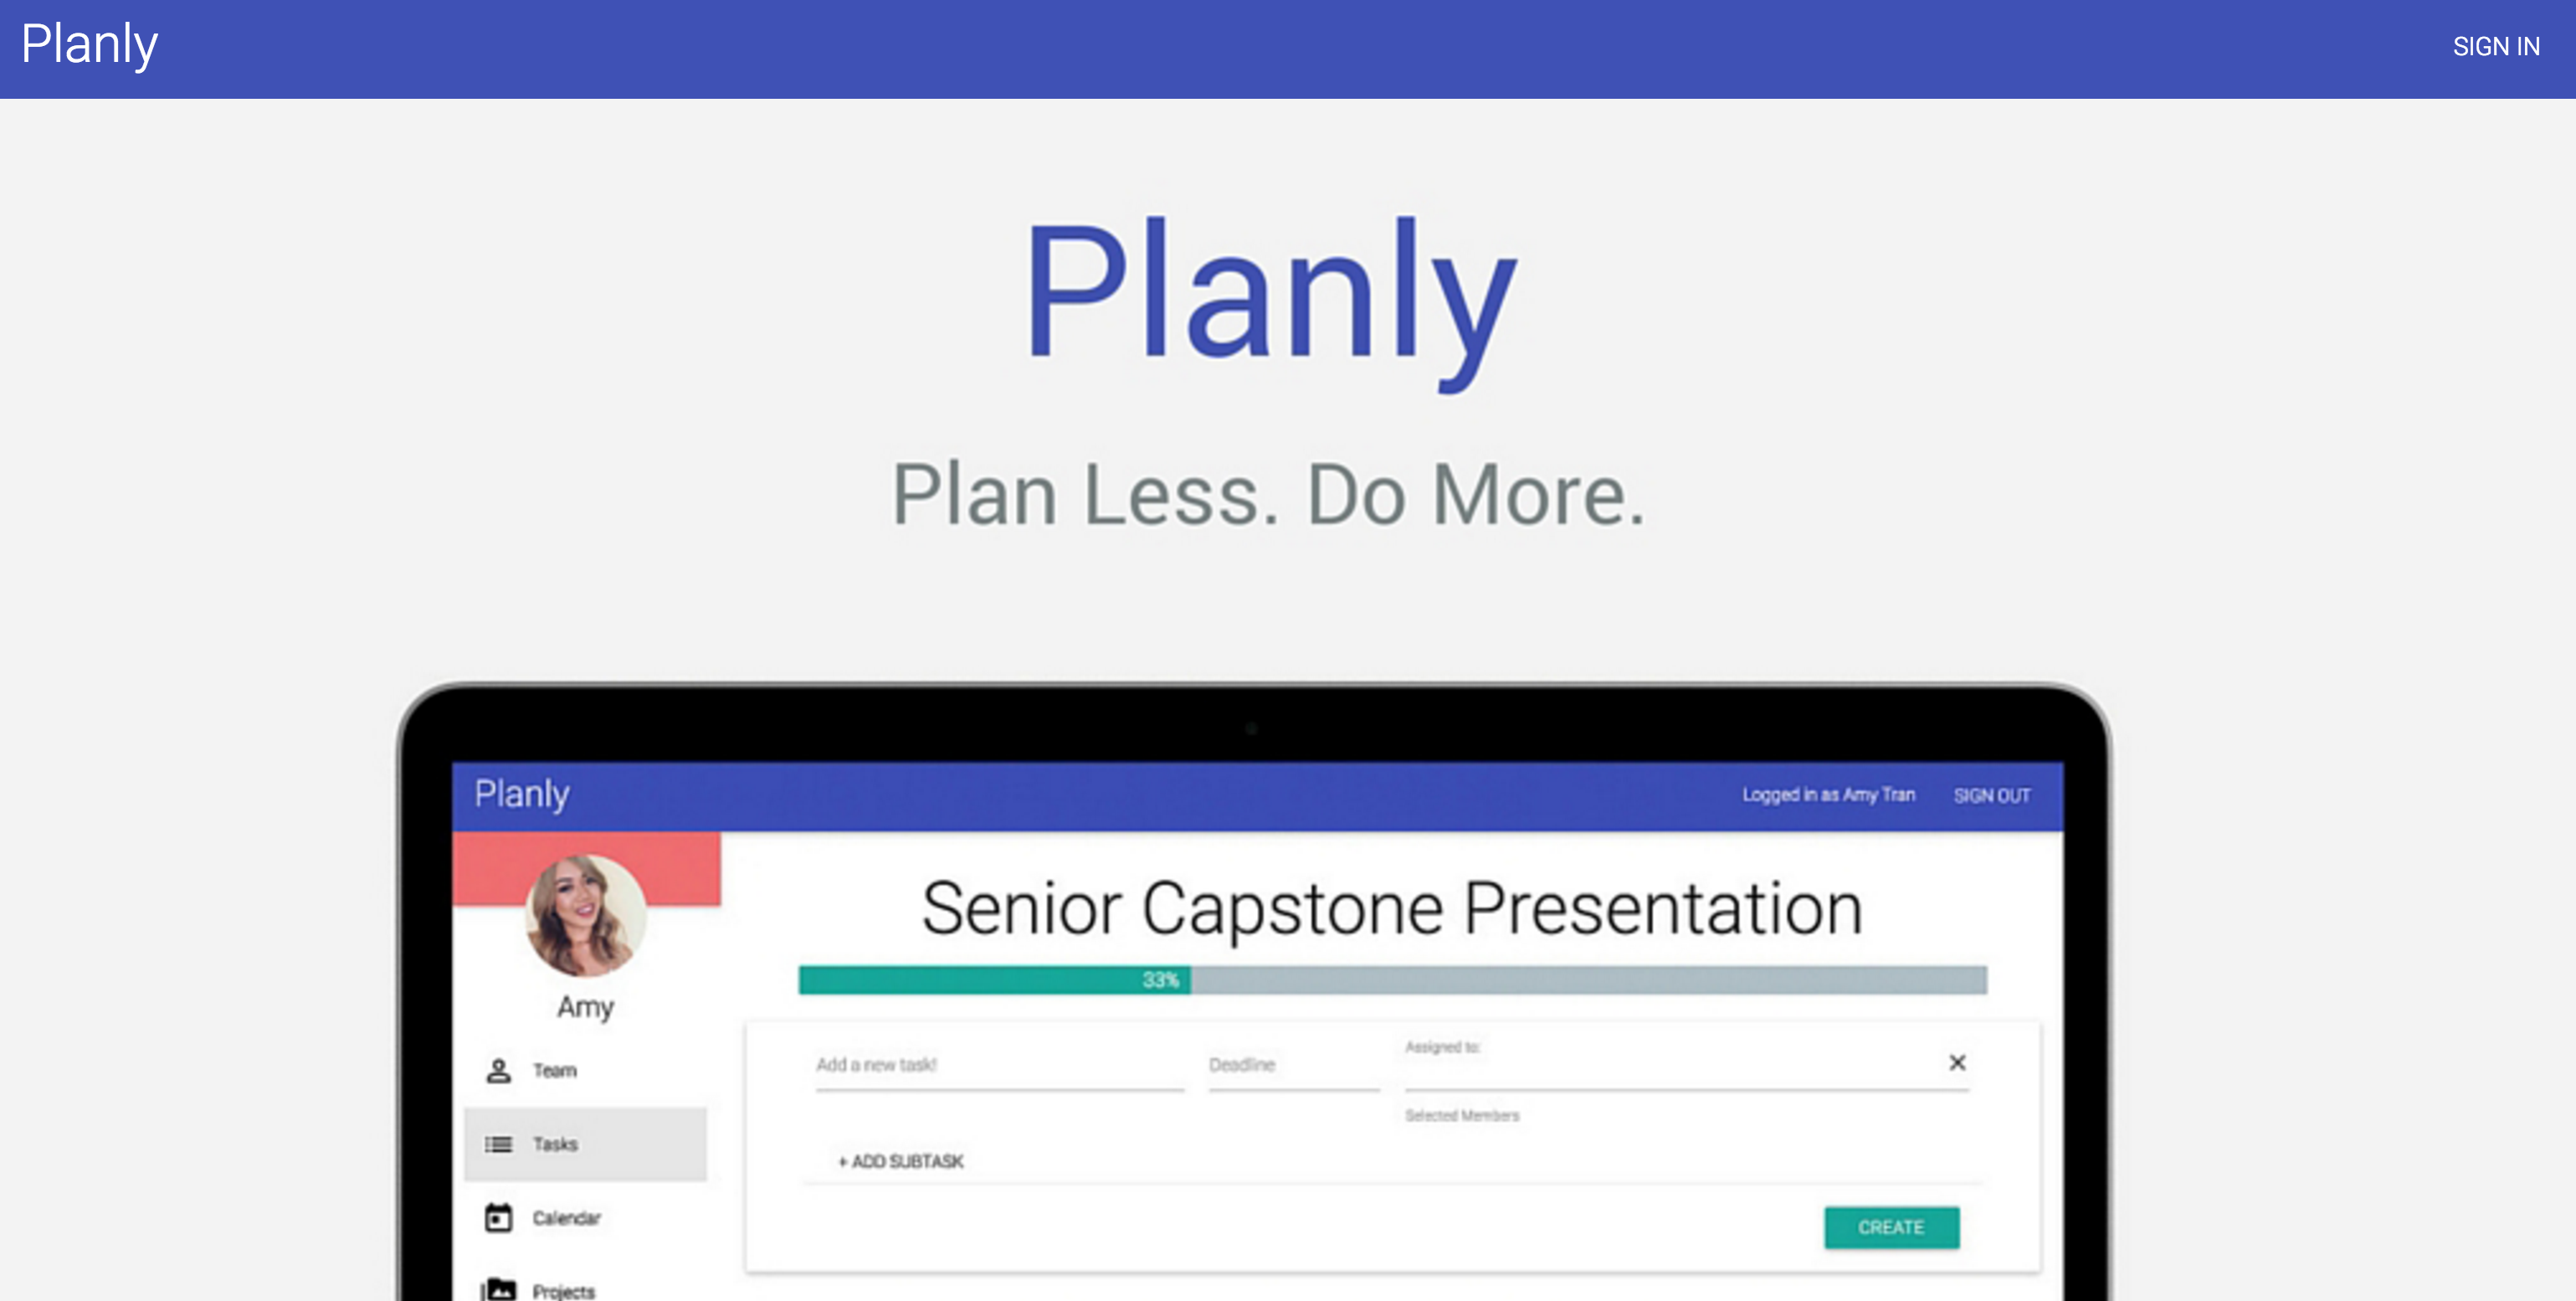
\includegraphics[width=\textwidth]{figure41.png}
\empuse{figure}
\caption{Homepage}
\label{homepage}
\end{figure}
\FloatBarrier

\subsection{Login}
In order to log in or sign up for \projectTitle, users must select ``Sign In'' on the top right corner of the homepage. We provide users with three different methods to sign up for an account: Google, Facebook, or Email, shown in \ref{signin}. After a user has successfully logged in, he/she will be presented with the \emph{Projects} view. The \emph{Projects} view, seen in \ref{projectview}, hosts all of the user's projects as well as the members for each project. 

\begin{figure}[ht]
\centering
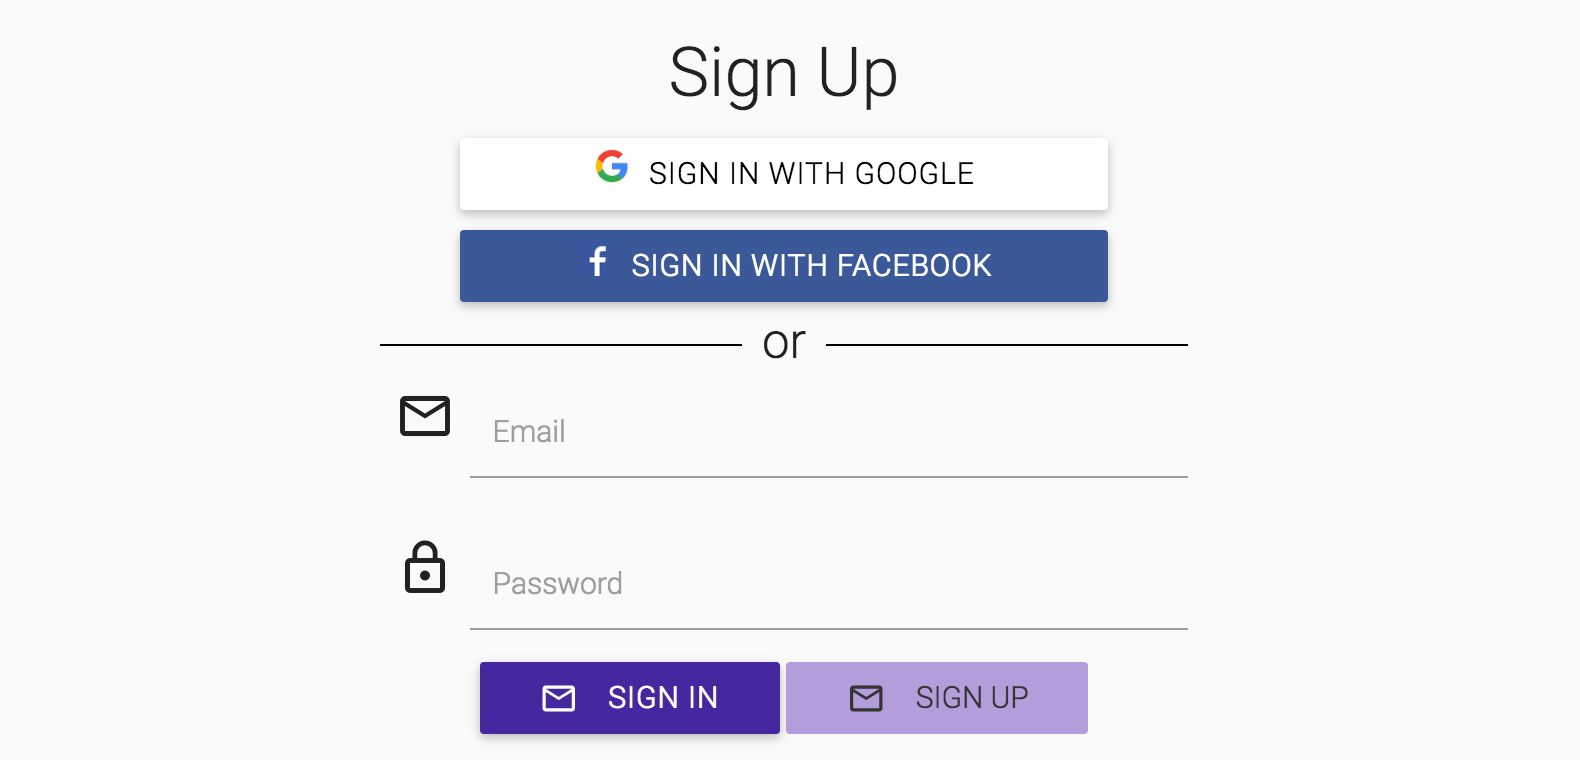
\includegraphics[width=\textwidth]{figure42.png}
\empuse{figure}
\caption{Sign In / Login Screen}
\label{signin}
\end{figure}
\FloatBarrier

\begin{figure}[ht]
\centering
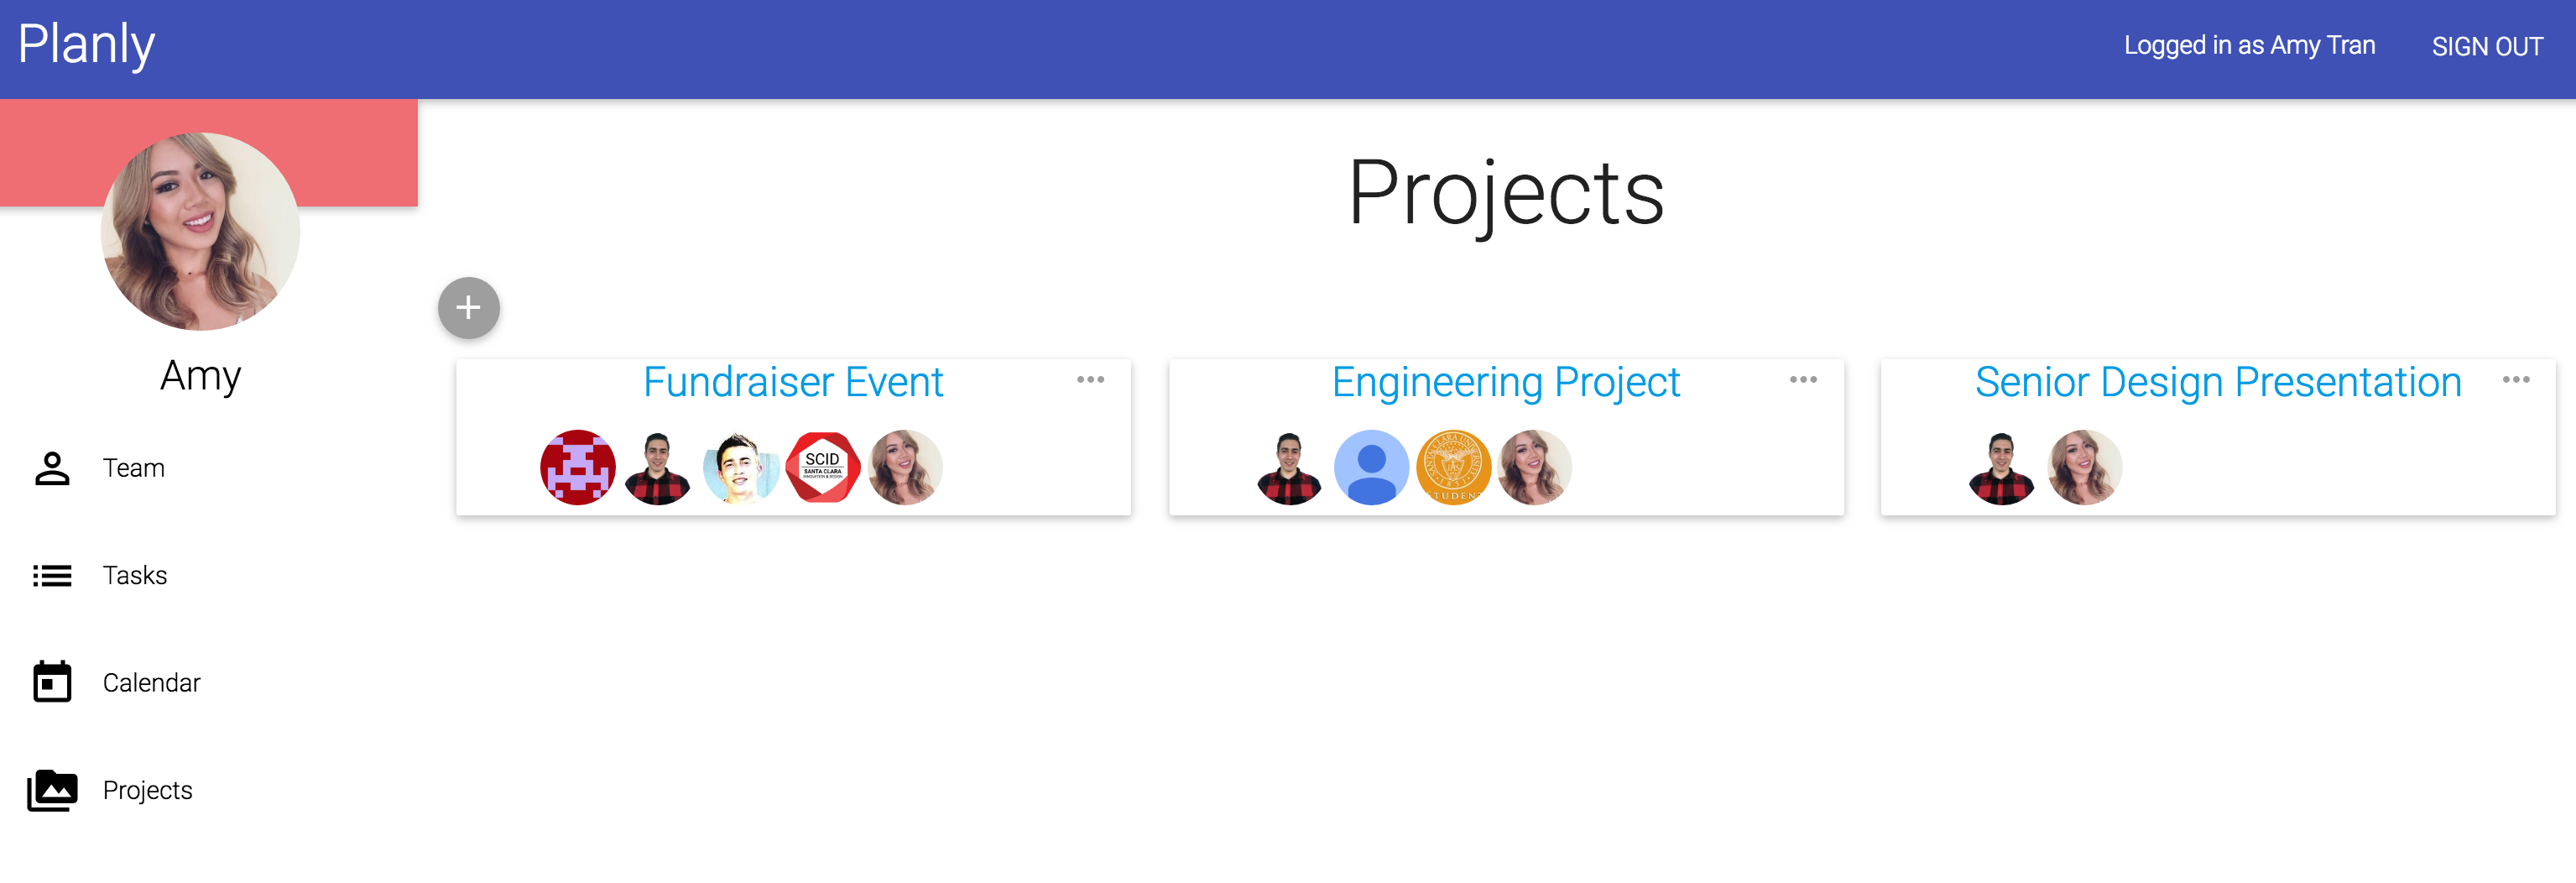
\includegraphics[width=\textwidth]{figure43.png}
\empuse{figure}
\caption{Projects View}
\label{projectview}
\end{figure}
\FloatBarrier

\subsection{Creating Projects and Teams}
From the \emph{Projects} view, users can create a new project as well as create teams for the project. By clicking on the + icon, users will activate the Project Creation form, depicted in \ref{projectcreationform}. The user needs to input the Project name, goal, deadline and team members. After completing the Project Creation form, users are given the option to create a team or to skip it at this time. 
\par If the user decides to create a team, he will need to enter the team name, description and team members.

\begin{figure}[ht]
\centering
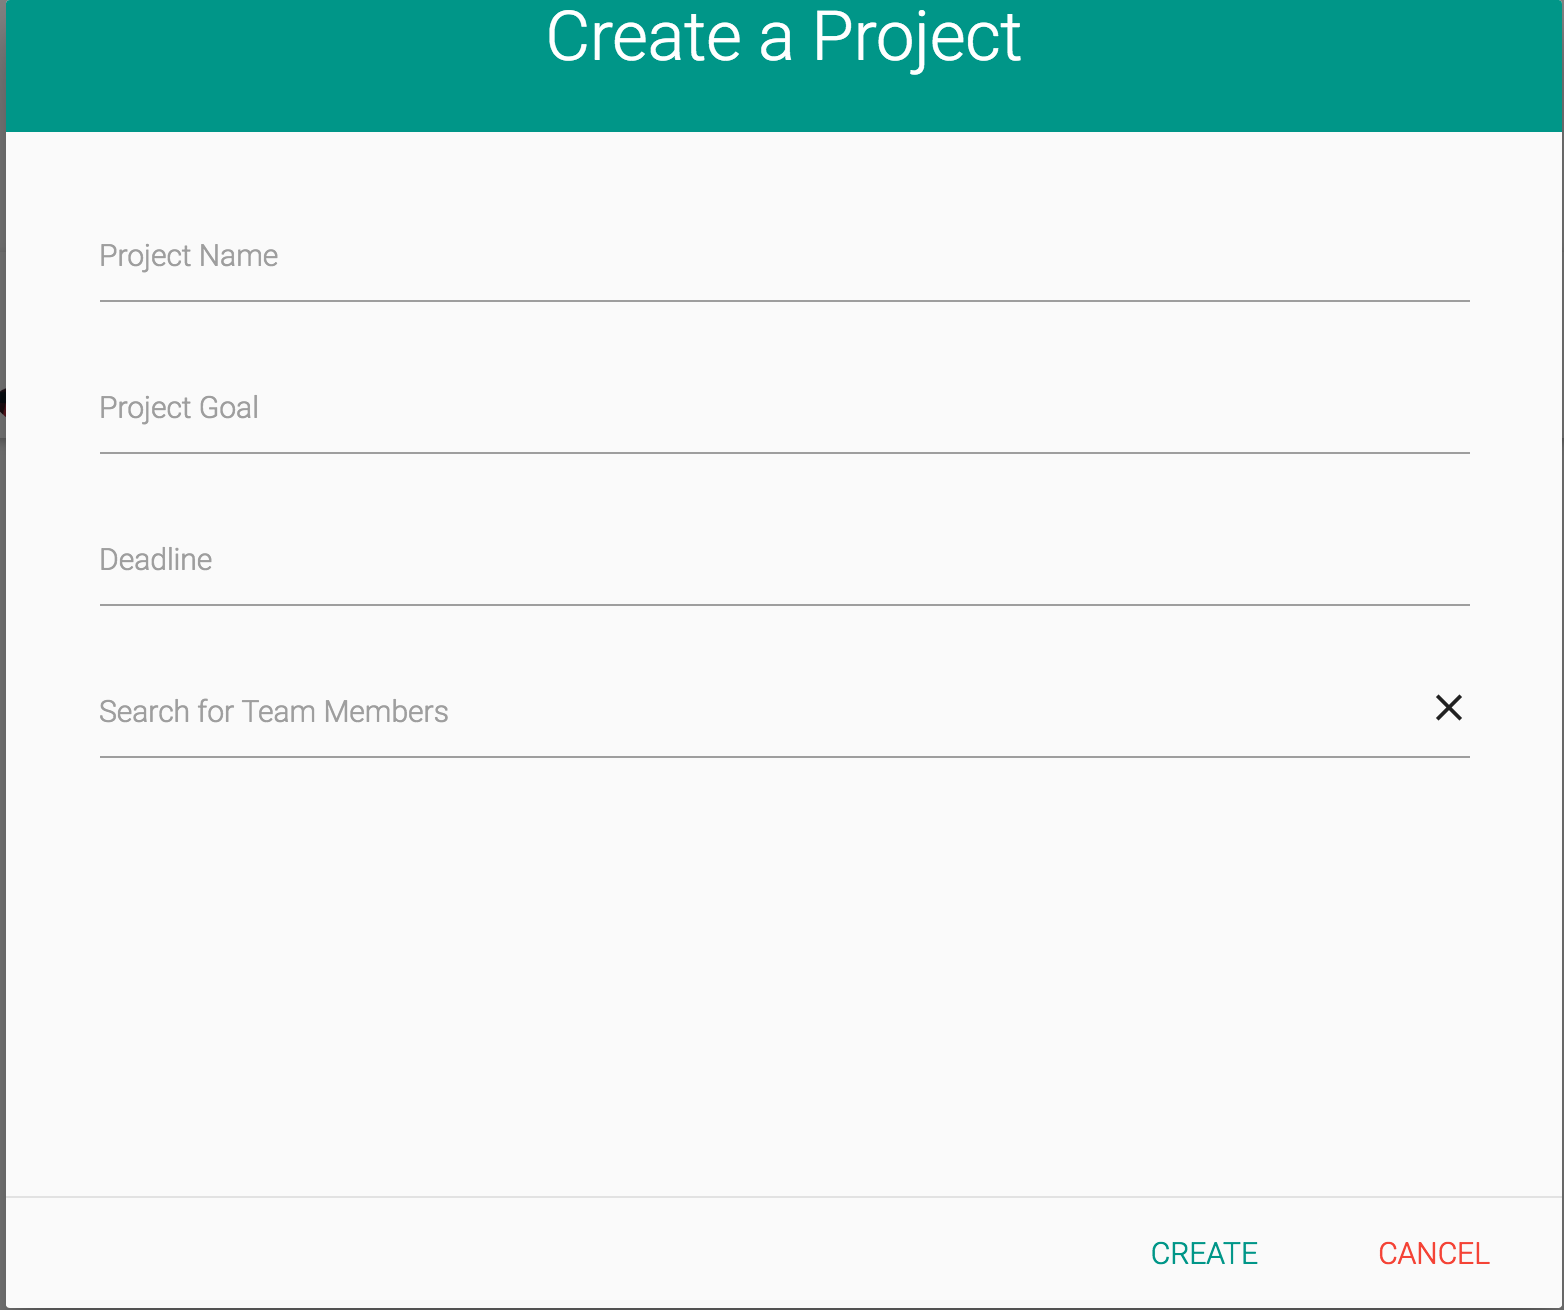
\includegraphics[width=\textwidth]{figure44.png}
\empuse{figure}
\caption{Project Creation Form}
\label{projectcreationform}
\end{figure}
\FloatBarrier

\subsection{Adding Tasks and Subtasks}
After the project has been created, users can now add task and subtask to the project. \ref{taskview} shows the \emph{Tasks} view. In the \emph{Tasks} view, users are presented with the project's name, progress bar, and a form to add tasks and subtasks. Once a user fills out the tasks form, he can then add a subtask or simply create the task. The task will appear on the screen with the task's deadline and who the task is assigned too. From there, users can click on the subtask icon to see the subtasks associated with the task or then can click the comment icon and post a comment. When a user marks a task as completed, the progress bar will change to reflect the progress of the project. 

\begin{figure}[ht]
\centering
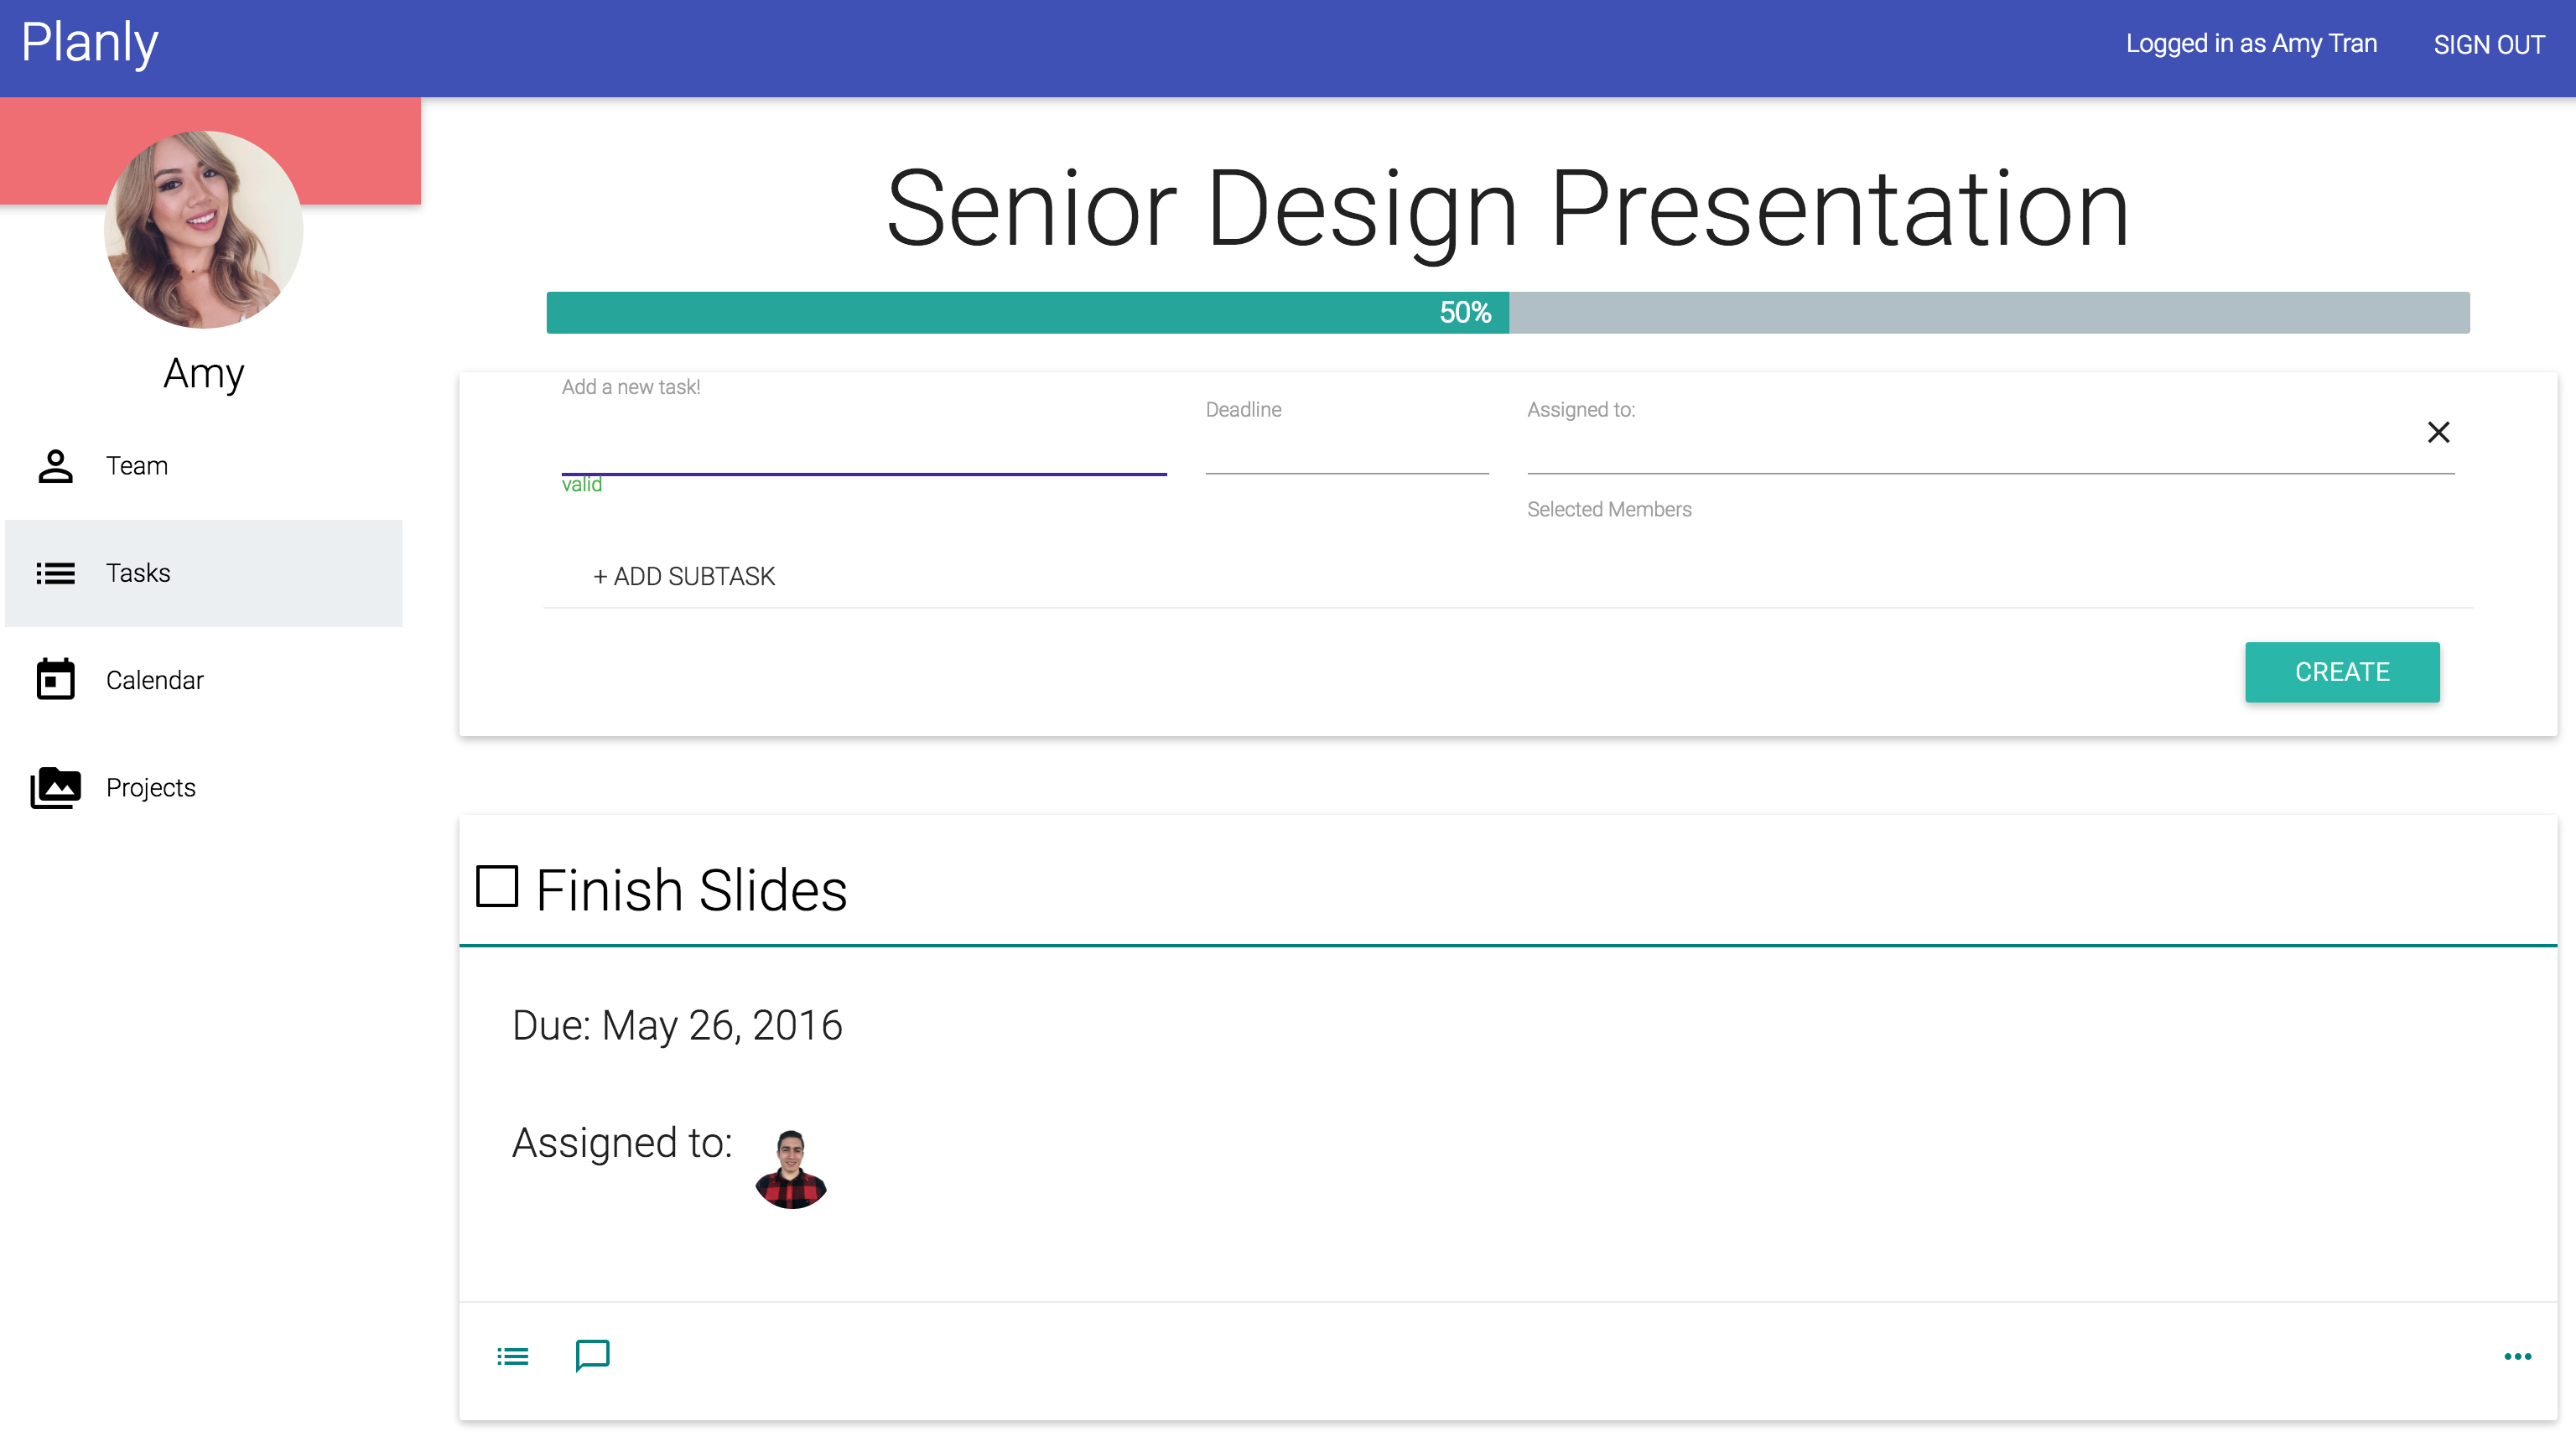
\includegraphics[width=\textwidth]{figure45.png}
\empuse{figure}
\caption{Task View}
\label{taskview}
\end{figure}
\FloatBarrier


\section{User Testing and Results}
After we completed \projectTitle, we hosted a user testing session where we invited students to complete a series of tasks and provide us with their feedback. At the end of the test, we asked users to submit an anonymous survey. Figure 4.6 and Figure 4.7 shows our user testing results. 
\par Beginning with the system as a whole, from the user testing results, the majority of the users found \projectTitle to be very usable system. To the question,``I found \projectTitle to be a usable system", 55.5\% of users rated \projectTitle as a 5, the highest score on our scale. As for the question `` I found \projectTitle to be overly complex", a third of the users rated \projectTitle a 1, meaning that they did not find \projectTitle to be complex. However, a third of the users also answered with a score of 3, thus although most users found \projectTitle to be usable, we acknowledge that there is still work to be done. 
\par Another question we asked in our survey was ``What are some areas of improvement for \projectTitle" and users were allowed to select all features that applied. According to the results, we found that the features that needed the most improvement were task and subtasks. It is interesting observation is that tasks and subtasks were the last features we worked on prior to the testing, thus it makes sense that these features were the weakest.  

\section{Lessons Learned}
We want to highlight three important lessons that we learned while developing \projectTitle: the importance of human centered design, the need for multiple system iterations, and the neccesity to integrate early and often.

\subsection{Challenges}
Had we not involved the user in the design of our system as early on as we did, we would have ended up in an entirely different place than we did. After completing our initial design and going through the design review, we took the advice provided to us and performed some user research before actually beginning development. The study exposed some major flaws in a lot of the interfaces we mocked up. This allowed to go back to the drawing board during the design phase rather than later on in the development phase. This lesson was so good, that we decided to borrow it moving forward. Each time we worked on a new feature, we would first mock it up, test it with users, and then implement it. 
\par We iterated through those steps repeatedly. Not only did this allow us to involve the user a lot more in the development of \projectTitle, it also enabled us to revisit some of the previous features we developed. As mentioned before, during our user testing we found that the features we implemented first generally had less issues than some of the newer features. Iteration is responsible for this. Each time we implemented a new feature, we were able to further test and correct the features that were already in place. 
\par As we added new features, we were not working on the same system, working on the same feature. We worked on our own systems, implementing different features in order to divide and conquer the development of \projectTitle. However, early on during development, if we spent too much time working on our own thing, we found that when the time came to finally merge our code, we had creeped into each others domains quite a bit. The solution was simple. Integrate early, and integrate often. By shortening the amount of time our code was apart, it prevented us from stepping on each others' toes and it also helped to ensure that any work performed by the other did not break any other part of the system. 

\subsection{Future Work}
Moving forward, we are looking to add more features, primarily pulling from the feedback we received through our user study. One feature that was frequentyly requested by users was the ability to edit teams. This leads us to believe that users want more overall control over the content of their projects. We will consider multiple ways to ensure they can customize their projects to their liking. Apart from the features reccommended in the user study, we also want to look at some of the features we weren't able to implement during our primary development, including, but not limited to, implementing calendar functionality which would allow users to import their event calendars in order to see who is available when and improving the functionality of the timeline so it better reflects the progress of the project by considering more factors than task completion. These features would greatly add to the user experience.
\par In order to ensure a better user experience forward, we need to consider more than just the features. We also need to optimize the application for scalability. This would mean that as we take on more users, the application wouldn't break due to the amount of traffic. We also need to increase the overall robustness of the application. As more users join \projectTitle, we are going to encounter more usage styles. This means more ways for people to encounter bugs. Ensuring we are as bug free as possible would increase the overall user experience. 
